\documentclass[reprint,amsmath,amssymb,aps,prb]{revtex4-2}




% \usepackage{graphicx}% Include figure files
\usepackage{dcolumn}% Align table columns on decimal point
\usepackage{bm}% bold math
\usepackage{hyperref}% add hypertext capabilities
% \usepackage{xcolor}

\usepackage{listings} % insert code fragments




\usepackage[T2A]{fontenc}                   %!? закрепляет внутреннюю кодировку LaTeX
\usepackage[utf8]{inputenc}                 %!  закрепляет кодировку utf8
\usepackage[russian, english]{babel}         %!  подключает русский и английский
\usepackage[margin=1.8cm]{geometry}         %!  фиксирует оступ на 2cm

% \usepackage[unicode, pdftex]{hyperref}      %!  оглавление для панели навигации по PDF-документу + гиперссылки

\usepackage{amsthm}                         %!  newtheorem и их сквозная нумерация
\usepackage{hypcap}                         %?  адресация на картинку, а не на подпись к ней
% \usepackage{caption}                        %-  позволяет корректировать caption 
\usepackage{fancyhdr}                       %   добавить верхний и нижний колонтитул
\usepackage{wrapfig}                        %!  обтекание таблиц и рисунков

\usepackage{amsmath}                        %!  |
\usepackage{amssymb,textcomp, esvect,esint} %!  |важно для формул 
\usepackage{amsfonts}                       %!  математические шрифты
\usepackage{mathrsfs}                       %  добавит красивые E, H, L
\usepackage{ulem}                           %!  перечеркивание текста
\usepackage{abraces}                        %?  фигурные скобки сверху или снизу текста
\usepackage{pifont}                         %!  нужен для крестика
\usepackage{cancel}                         %!  аутентичное перечеркивание текста
\usepackage{esvect}                         %  добавит вектора стрелочками

\usepackage{graphicx}                       %?  графическое изменение текста
\usepackage{indentfirst}                    %   добавить indent перед первым параграфом
\usepackage{xcolor}                         %   добавляет цвета
\usepackage{enumitem}                       %!  задание макета перечня.

\usepackage{booktabs}                       %!  добавляет книжные линии в таблицы
% \usepackage{multirow}                       %   объединение ячеек в таблицах
% \usepackage{tikz}                           %!  высокоуровневые рисунки (кружочек)
% \usepackage{import}                         %   |
% \usepackage{xifthen}                        %   |
% \usepackage{pdfpages}                       %   | вставка рисунков pdf_tex
% \usepackage{transparent}                    %   |

\usepackage{bbm}                            %   добавляет \mathbbm{1}



% \definecolor{grey}{HTML}{666666}
% \definecolor{ublue}{HTML}{08088A}
% \definecolor{linkcolor}{HTML}{0000CC}
% \definecolor{urlcolor}{HTML}{006600}
% \hypersetup{
%     pdfstartview=FitH,  
%     linkcolor=linkcolor,
%     urlcolor=urlcolor, 
%     colorlinks=true,
%     citecolor=blue}
% базовая подстройка
\renewcommand{\d}{\, d}
\renewcommand{\leq}{\leqslant}
\renewcommand{\geq}{\geqslant}


% tmp
\newcommand{\tn}[1]{(\textbf{#1})}
\newcommand{\nBF}{n_\text{\scalebox{0.7}{BF}}}
\newcommand{\Hc}{\sub{h}{c}}
\newcommand{\Z}{\mathcal{Z}}
\newcommand{\Kc}{\sub{K}{c}}
\newcommand{\gs}{\ket{\textnormal{gs}}}
\newcommand{\F}{\mathcal{D}}

% авторские команды
\newcommand{\vc}[1]{\boldsymbol{#1}}
\newcommand{\1}{\mathbbm{1}}
\newcommand{\T}{^{\textnormal{T}}}
\newcommand{\D}{^{\dag}}
\newcommand{\sub}[2]{#1_{\textnormal{#2}}}
\newcommand{\vp}{\vphantom{\dfrac{1}{2}}}
\newcommand{\hc}{\textnormal{h.c.}}

% операторы (просто прямой текст)
\renewcommand{\Im}{\mathop{\mathrm{Im}}\nolimits}
\renewcommand{\Re}{\mathop{\mathrm{Re}}\nolimits}
% \renewcommand{\P}{\mathop{\mathrm{P}}\nolimits}
% \newcommand{\E}{\mathop{\mathrm{E}}\nolimits}
% \newcommand{\D}{\mathop{\mathrm{D}}\nolimits}
% \newcommand{\cov}{\mathop{\mathrm{cov}}\nolimits}
\newcommand{\diag}{\mathop{\mathrm{diag}}\nolimits}
\newcommand{\card}{\mathop{\mathrm{card}}\nolimits}
\newcommand{\grad}{\mathop{\mathrm{grad}}\nolimits}
\renewcommand{\div}{\mathop{\mathrm{div}}\nolimits}
\newcommand{\rot}{\mathop{\mathrm{rot}}\nolimits}
\newcommand{\Ker}{\mathop{\mathrm{ker}}\nolimits}
\newcommand{\spec}{\mathop{\mathrm{spec}}\nolimits}
\newcommand{\sign}{\mathop{\mathrm{sign}}\nolimits}
\newcommand{\tr}{\mathop{\mathrm{tr}}\nolimits}
\newcommand{\rg}{\mathop{\mathrm{rg}}\nolimits}
\newcommand{\const}{\textnormal{const}}


\renewcommand{\th}{\mathop{\mathrm{tanh}}\nolimits}
\newcommand{\sh}{\mathop{\mathrm{sinh}}\nolimits}
\newcommand{\ch}{\mathop{\mathrm{cosh}}\nolimits}

% цветной текст
\newcommand{\red}[1]{\textcolor{red}{#1}}
\newcommand{\green}[1]{\textcolor{urlcolor}{#1}}
\newcommand{\blue}[1]{\textcolor{ublue}{#1}}


% символы
\newcommand{\cmark}{\text{\ding{51}}}
\newcommand{\xmark}{\text{\ding{55}}}


% подгрузка pdf_tex картинок
% \newcommand{\incfig}[1]{%
%     \def\svgwidth{\columnwidth}
%     \import{./figures/}{#1.pdf_tex}
% }


% специфично к квантам
\newcommand{\ket}[1]{\left| #1 \right\rangle}
\newcommand{\bra}[1]{\left\langle #1 \right|}

% \newcommand{\dppp}{\frac{d^3 p}{(2 \pi \hbar)^3}}

\DeclareDocumentCommand{\bk}{m o m}{
    \IfNoValueTF{#2}{\langle #1 | #3 \rangle}{\langle #1 | #2 | #3 \rangle}
}

\DeclareDocumentCommand{\kb}{m o m}{
    \IfNoValueTF{#2}{| #1 \rangle \langle #3 |}{| #1 \rangle #2 \langle #3 |}
}


% снимаю шляпу
% \renewcommand{\hat}[1]{#1}


\lstdefinestyle{mystyle}{
    backgroundcolor=\color{backcolour},   
    commentstyle=\color{codegreen},
    keywordstyle=\color{magenta},
    numberstyle=\tiny\color{codegray},
    stringstyle=\color{codepurple},
    basicstyle=\ttfamily\footnotesize,
    breakatwhitespace=false,         
    breaklines=true,                 
    captionpos=b,                    
    keepspaces=true,                 
    numbers=left,                    
    numbersep=5pt,                  
    showspaces=false,                
    showstringspaces=false,
    showtabs=false,                  
    tabsize=2
}

\lstset{style=mystyle}



\begin{document}


\title{Quantum Phase Transitions in the 1D Bose-Hubbard Model with DMRG}

\author{Kirill Khoruzhii}
\affiliation{Technische Universität München, Max-Planck-Institut für Quantenoptik}

\date{\today}% It is always \today, today,
             %  but any date may be explicitly specified

\begin{abstract}
This study investigates quantum phase transitions in the 1D Bose-Hubbard model. Noted for its Mott insulator (MI) and superfluid (SF) phases, the model is analyzed using Density Matrix Renormalization Group (DMRG) methods. The correlation length $\xi$ and average site occupancy $\langle n_j \rangle$ are examined. Our findings indicate that in the MI phase, particle mobility is suppressed and $\Gamma(r)$ decays exponentially, whereas in the SF phase, particles are delocalized, leading to polynomial decay. We also explore the impact of bond dimension $D$ in DMRG, noting that small $D$ yields mean-field-like solutions.
\end{abstract}


% MI-SF_QPT

\maketitle

The investigation of quantum phase transitions in strongly correlated systems is an important and fascinating area of research. The one-dimensional Bose-Hubbard model is a minimal bosonic many-particle model that captures the essential physics of interacting bosons on a lattice \cite{kuehner_phases_1998}
\begin{equation*}
	H = -t \sum_{j} (a_j\D a_{j+1} + \hc) + \tfrac{1}{2}U \sum_j n_j (n_j-1) - \mu \sum_j n_j
\end{equation*}
and garnered significant attention due to the existence of both the Mott insulator (MI) and superfluid (SF) phases, as well as the successful application of DMRG \cite{PhysRevLett.69.2863}.

The MI\textsuperscript{\footnote{
    The MI phase is particularly notable for its role in ultracold atom experiments, where it facilitates the deterministic preparation of a single-site occupancy lattice—a critical step in quantum simulation and computation experiments \cite{choi_exploring_2016}.
}} phase is characterized by its lack of particle mobility due to strong interactions, resulting in a fixed integer number of particles per site and an energy gap for particle-hole excitations. This phase exhibits suppressed number fluctuations and localized particles, leading to short correlation lengths and an insulating behavior. In the MI phase, the correlation function $\Gamma(r) = \langle a_j^\dagger a_{j+r} \rangle$ decays \textit{exponentially} with distance (fig. \ref{fig:decay}.1). 

On the other hand, the SF phase features delocalized particles that can move freely across the lattice, leading to long-range phase coherence and the absence of an energy gap. This phase is marked by large number fluctuations and a diverging correlation length, indicating a coherent, macroscopic quantum state. In the SF phase, the correlation function $\Gamma(r)$ decays \textit{polynomially} with distance (fig. \ref{fig:decay}.3).


\begin{figure}[b]
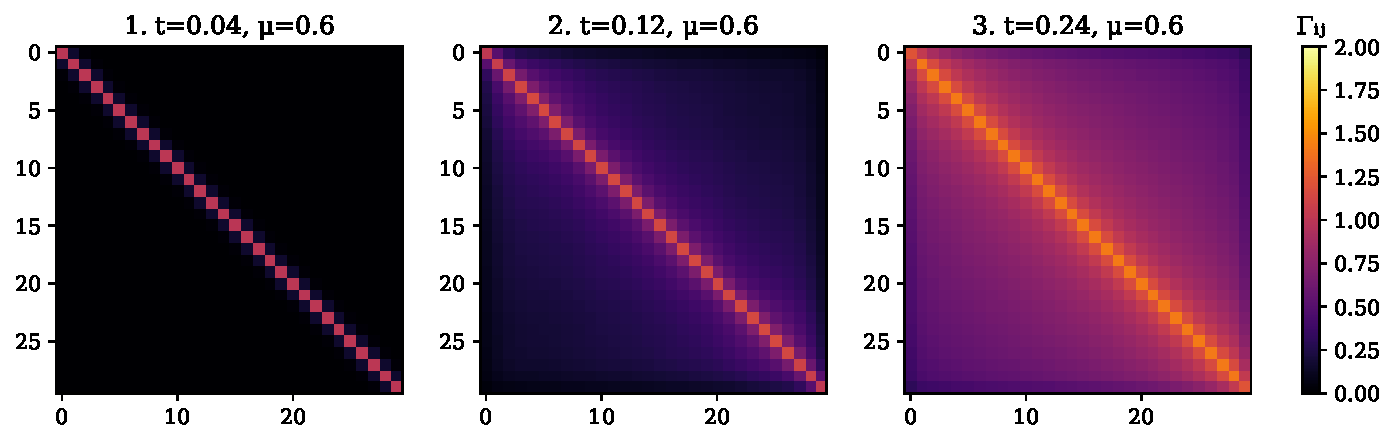
\includegraphics[width=\linewidth]{imgs/corrs.pdf}
\caption{The characteristic form of $\Gamma_{ij}$ at three points in the phase space: MI (1), critical point (2), and SF (3). The same points are used for illustration purposes throughout the text.}
\label{fig:corrmat}
\end{figure}

\section{Methodology}


In this article, we will focus on three key quantities to distinguish between these phases: the correlation length $\xi$, the average site occupancy $\langle n_j \rangle$, and the polynomial degree \( K \) with which \(\Gamma^2\) decays, following the approach in [1]. These properties provide valuable insights into the nature of the MI and SF phases. By examining these parameters, we aim to deepen our understanding of the phase transitions within the one-dimensional Bose-Hubbard model.





We use finite-size DMRG \cite{catarina_density-matrix_2023, Fishman_2022}, with the primary results presented for a lattice with $L=30$ sites, a cutoff $\sub{n}{c} = 5$, open boundary conditions, and a bond dimension $D=300$ (unless otherwise specified). Fixing $U=1$, we examine the system's behavior in the $(t, \mu)$-plane\textsuperscript{\footnote{
     The parameter $t$ represents the hopping amplitude between neighboring sites, $U$ denotes the on-site interaction strength, and $\mu$ is the chemical potential controlling the particle number.
}}.


\begin{figure}[t]
    \centering
    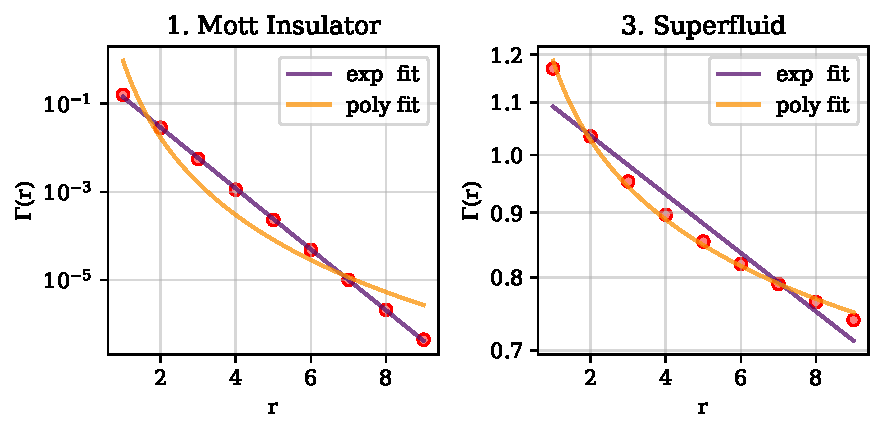
\includegraphics[width=\linewidth]{imgs/decay.pdf}
    \caption{Demonstration of the exponential decay of $\Gamma(r)$ for MI (1) and polynomial decay for SF (3).}
    \label{fig:decay}
\end{figure}


\begin{figure}[b]
    \centering
    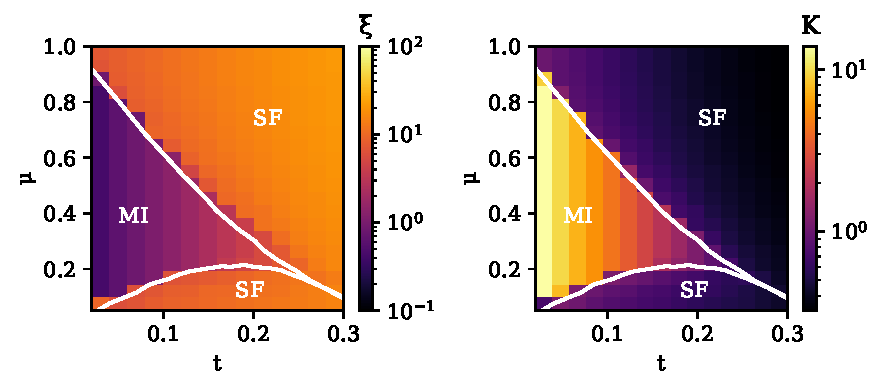
\includegraphics[width=\linewidth]{imgs/phases2.pdf}
    \caption{Phases of the 1D Bose-Hubbard model. Phase boundaries are drawn according to the results from \cite{kuehner_phases_1998}. Near the boundaries, the divergence of $\xi$ and the approach of $K$ to the critical value $\sub{K}{c}=1/2$ can be observed.}
    \label{fig:phases2}
\end{figure}





\begin{figure*}
    \centering
    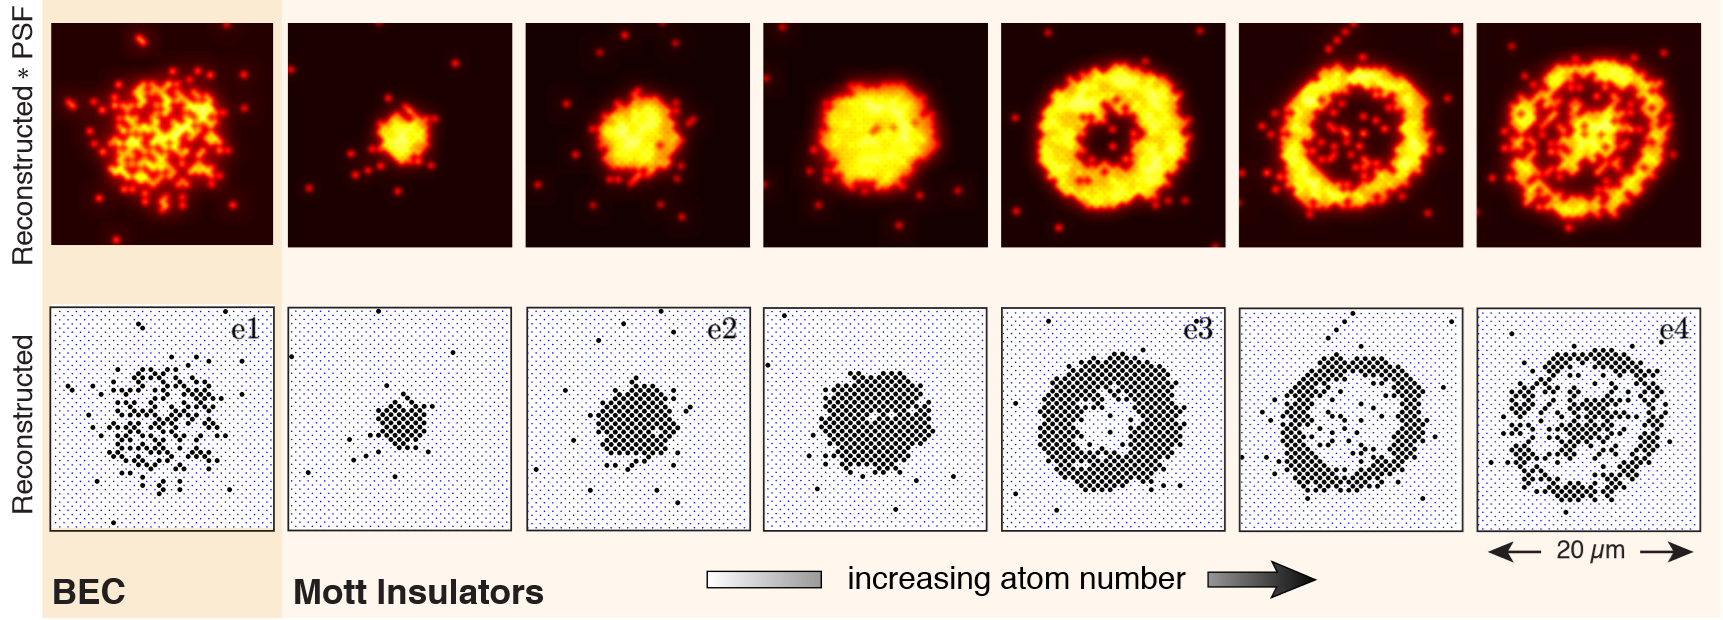
\includegraphics[width=\textwidth]{imgs/MIexp.png}
    \caption{High-resolution fluorescence images of a BEC (SF) and Mott insulators (MI) with in-plane harmonic confinement from \cite{sherson_single-atom-resolved_2010}. Experimentally obtained images of a BEC (e1) and Mott insulators for increasing particle numbers (e2, e3, e4) in the zero-tunneling limit, showing $\langle n_j \rangle \mod 2$. Clear integer filling of the lattice with $n=1, 2, 3$ can be observed.}
    \label{fig:MIexp}
\end{figure*}



Through $\xi$ and $K$, we can obtain information about particle mobility and correlations. A  correlation length larger $\xi$ signifies longer-range correlations, indicating the extent of coherence in the system, typical in the superfluid phase, while a smaller $\xi$ indicates short-range correlations, characteristic of the Mott insulator phase. 

The correlation length can be determined in two ways: first, by definition,
\begin{equation*}
	\xi(r) = \frac{\sum_r r^2 \Gamma(r)}{\sum_r \Gamma(r)},
\end{equation*}
although this approach is more sensitive to the finite size of the system. Alternatively, assuming an exponential decay $\sub{\Gamma}{MI}(r) \propto e^{-r/\xi}$, $\xi$ can be found through fitting the calculated correlator, which works well in the MI region. Similarly, by fitting the decay in the SF and critical regions, where we expect a polynomial decay, we can determine the exponent $K$ via $\sub{\Gamma}{SF}^2(r) \propto r^{-K}$. The results of fitting\textsuperscript{\footnote{
  One could assume that the function $e^{-r/\xi} / r^{K/2}$ would describe the decay well across the entire phase space. However, such a fit is more unstable, and the phases can still be distinguished throughout the space by either $K$ or $\xi$.
}} with these two functions are presented in Fig. \ref{fig:decay}, where it is evident that the decay is exponential for MI and polynomial for SF
% \textsuperscript{\footnote{
% 	One could assume that the function $e^{-r/\xi} / r^{K/2}$ would describe the decay well across the entire phase space. However, such a fit is more unstable, and the phases can still be distinguished throughout the space by either $K$ or $\xi$.
% }}.

Additionally, the average number of particles per site $\langle n_j \rangle$ is a crucial indicator of the MI phase. In the MI phase, $\langle n_j \rangle$ is typically an integer (fig. \ref{fig:MIexp}), reflecting the fixed number of particles due to strong repulsive interactions, when particle mobility is suppressed, and the system is incompressible. In contrast, in the superfluid phase, $\langle n_j \rangle$ can vary continuously, indicating higher particle mobility and the absence of a gap for particle-hole excitations. To quantify the deviation from integer filling, we introduce $\delta n_j = n_j - 1$, which helps in analyzing the fluctuations and transitions between the phases.




\section{Phase Diagram}

For $t \in[0, 0.3]$ in steps of $0.02$ and $\mu \in [0, 1]$ in steps of $0.05$ at $U=1$, the correlators $\Gamma_{ij}$ were calculated. From these, the values of $\xi$ and $K$ were obtained through fitting, and the results are presented in Fig. \ref{fig:phases2}. The correlation length exhibits a sharp divergence near the critical point $\ln \xi \sim 1 / \sqrt{t_c - t}$ 
subject to finite size limitations. The critical exponent $\sub{K}{c}$ of the phase transition is also known from Luttinger liquid theory \cite{PhysRevB.46.9325,kuehner_phases_1998}. At the BKT transition with $\langle n_j \rangle = 1$, $K$ is expected to be $\sub{K}{c} = 1/2$. However, even without this knowledge, it is quite possible to distinguish the two regions based on $K$. In this context, Luttinger liquid theory simply helps to define this boundary more precisely. The divergence of $\xi$ and the critical value $K = \sub{K}{c}$ are in complete agreement with the phase boundaries defined in \cite{kuehner_phases_1998}.


\begin{figure}[b]
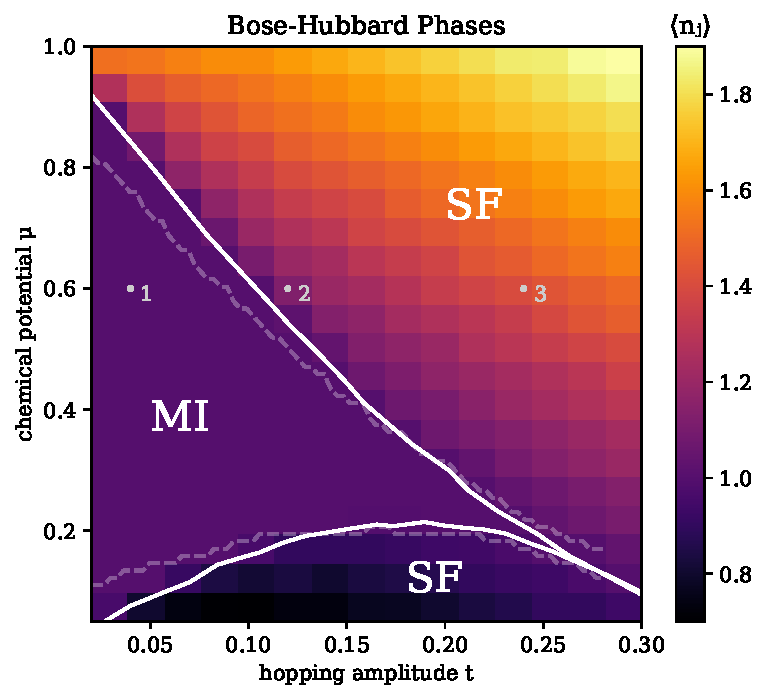
\includegraphics[width=0.9\linewidth]{imgs/phases.pdf}
\caption{The average number of particles per site. It is evident that the filling is strictly one in the MI region.}
\label{fig:phases}
\end{figure}


\begin{figure*}[t]
    \centering
    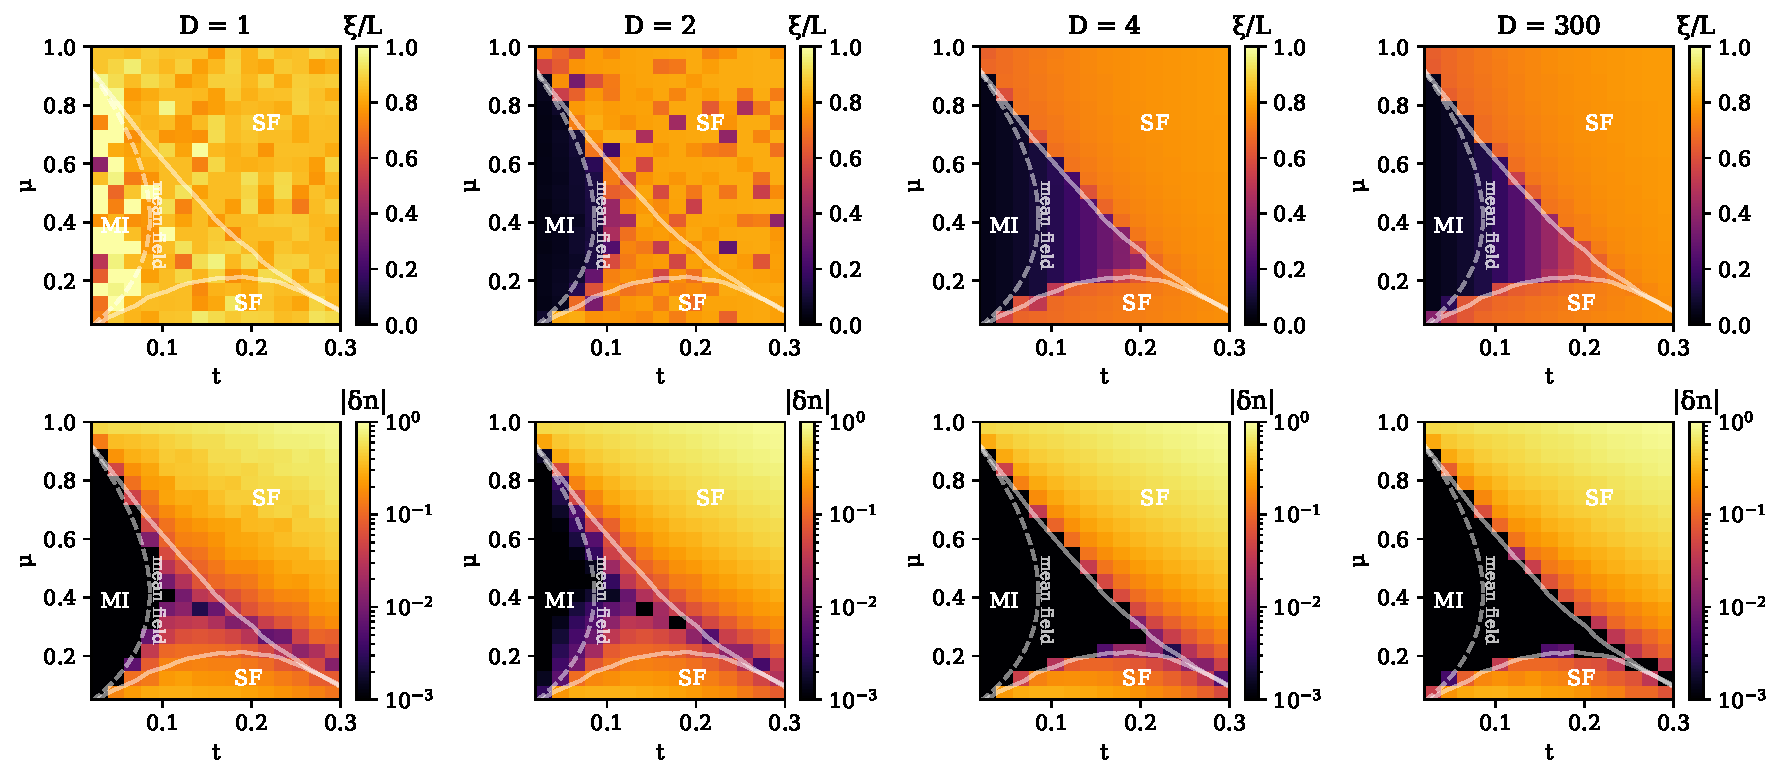
\includegraphics[width=\textwidth]{imgs/phases2mf.pdf}
    \caption{Phase diagrams obtained via DMRG for various bond dimensions $D$. As $D$ decreases, the solution approaches the mean field solution, both in terms of system filling and correlation length.}
    \label{fig:mf}
\end{figure*}


Note that the diagonal part of the calculated correlators $\Gamma_{jj} = n_j$, and by plotting $\langle n_j\rangle$ in the $(t, \mu)$-plane, we can clearly observe the unit filling in the MI phase (Fig. \ref{fig:phases}). The characteristic points 1, 2, and 3 used earlier for illustration are also marked here. Using linear interpolation with smoothing, we have also delineated the boundaries of the $\langle n_j\rangle = 1$ region (white dashed line), which closely align with the phase boundaries. In the SF region, increasing $\mu$ leads to a continuous and monotonic increase in the average number of particles.





\section{XX-model and mean-field from DMRG}


It is important to consider the approximations we make in DMRG calculations. For instance, what happens if the bond dimension $D$ is not sufficiently large? In the limit of $D=1$, we obtain a mean field solution \cite{PhysRevB.40.546}, with the phase boundary defined by:
\begin{equation*}
	1 + 2t \left(\tfrac{1}{-\mu} + \tfrac{2}{\mu-U}\right) = 0.
\end{equation*}
However, with $D=4$, we start to see the characteristic elongated shape of the MI region (Fig. \ref{fig:mf}).

In the limit of $\sub{n}{c}=1$, we obtain hard-core bosons, which, through the Jordan-Wigner transformation, correspond to the XX model  with paramagnetic and ferromagnetic phases. These phases are also characterized by exponential and polynomial decays, respectively. This gives a characteristic phase boundary $\mu=2t$ for $\mu, t \ll U$, where $\mu$ acts as an external magnetic field \cite{Mbeng_2024}.


% \section{Acknowledgements}


I would like to express my gratitude to Trofim Ruzaikin and Mikhail Goloshchapov for their valuable advice and inspiration in exploring this topic.


\bibliography{DMRG}

\newpage


\appendix

\section{MPO Representation of the Hamiltonian}

Following \cite{catarina_density-matrix_2023}, we can express the 1D Bose-Hubbard Hamiltonian with several terms:
\begin{align*}
	&\ldots \overset{4}{\otimes} \1 \overset{4}{\otimes} - t \hat{a}^\dagger \overset{2}{\otimes} \hat{a} \overset{1}{\otimes} \1 \overset{1}{\otimes} \ldots \\
	&\ldots \overset{1}{\otimes} \1 \overset{4}{\otimes} -t \hat{a} \overset{3}{\otimes} \hat{a}^\dagger \overset{1}{\otimes} \1 \overset{1}{\otimes} \ldots \\
	&\ldots \overset{1}{\otimes} \1 \overset{4}{\otimes} \phantom{-t} \hat{c} \phantom{\D} \overset{1}{\otimes} \1 \phantom{\D} \overset{1}{\otimes} \1 \overset{1}{\otimes} \ldots
\end{align*}
where the operator $\hat{c}$ is defined as:
\begin{equation*}
	\hat{c} = \tfrac{1}{2}U \hat{n}^2 - \left(\mu + \tfrac{U}{2}\right) \hat{n}_j.
\end{equation*}
Thus, we can write our Hamiltonian as an MPO of the form:
\begin{equation*}
	\hat{H} = \begin{pmatrix}
		\1 & 0 & 0 & 0 \\
		\hat{a} & 0 & 0 & 0 \\
		\hat{a}^\dagger & 0 & 0 & 0 \\
		\hat{c} & -t \hat{a}^\dagger & -t \hat{a} & \1 \\
	\end{pmatrix}.
\end{equation*}

For $L=4$, it has been verified that the Hamiltonian obtained from the MPO matches the explicitly written Hamiltonian. Additionally, using Exact Diagonalization (ED), it was confirmed that the ground states obtained from both methods are consistent.





% \newpage \phantom{42} \newpage

\begin{widetext}
\section{Code listing: Julia} \label{app:codesP}

The calculation of the ground state of the system can be implemented using DMRG in Julia and the ITensor package \cite{Fishman_2022}, which was convenient for verifying the correctness of the implementation on larger system sizes.
\begin{lstlisting}[language=Python]
using NPZ
using ITensors
using ITensorMPS


function calculate_adagacorr(L, mu, U, J, nsweeps, maxdim, cutoff, bc, nc)
    file_name = "data/J$(round(Int,100*J))_mu$(round(Int,100*mu))_L$(L)_bc$(bc)_nc$(nc)_sweeps$(nsweeps)_dim$(maxdim[1]).npy"
    println("processing $(file_name[6:end-4])")
    
    # Initialize the sites
    sites = siteinds("Boson", L; dim=5, conserve_qns=false)

    # Define the operator sum
    os = OpSum()
    for b in 1:(L - 1)
        os += -mu - U*0.5, "N", b
        os += U*0.5, "N", b, "N", b
        os += -J, "A", b, "Adag", b + 1
        os += -J, "Adag", b, "A", b + 1
    end
    os += -mu - U*0.5, "N", L
    os += U*0.5, "N", L, "N", L
    if bc == 1
        os += -J, "A", 1, "Adag", L
        os += -J, "Adag", 1, "A", L
    end

    # Construct the Hamiltonian as an MPO
    H = MPO(os, sites)

    # Initialize a random MPS
    psi0 = randomMPS(sites)
    
    # Run DMRG to find the ground state
    energy, psi = dmrg(H, psi0; nsweeps, maxdim, cutoff)

    # Calculate the correlation matrix
    adagacorr = correlation_matrix(psi, "Adag", "A")
    npzwrite(file_name, adagacorr)

    return adagacorr, psi, energy
end
\end{lstlisting}
\end{widetext}


% \newpage \phantom{42} \newpage

% \begin{widetext}
\section{Code} \label{app:codesP}

Код для получения диффузного расстояния на кубике 222. Для $\sub{K}{max} = 30$ кривая с fig. \ref{fig:2} считается за 2 минуты, для $\sub{K}{max} = 50$ за 9 минут. В примере $k=10^{8}$ и резудьтат усредняется $\text{rep}=10$ раз.

\begin{lstlisting}[language=Python]
import torch

neighbors = ... # torch.tensor
distance  = ... # torch.tensor
ds        = torch.unique(distance)
N         = neighbors.size(0)

def get_pilgrims_position(L, k=100_000):
    pilgrims_position = torch.zeros(k, dtype=torch.int64, device=device) 
    for j in range(L):
        pilgrims_position = torch.gather(
            neighbors[pilgrims_position], 
            1, 
            torch.randint(6, (k,), device=device).view(k, 1)
        ).squeeze(1)
    return pilgrims_position

def get_D(Kmax, k=100_000_000, rep=10):
    Ks = torch.arange(1, Kmax+1, device=device)
    visited = torch.zeros((neighbors.size(0), Kmax), dtype=torch.int64, device=device)
    
    for R in tqdm(range(rep)):
        for (j, K) in enumerate(Ks):
            pilgrims_position = get_pilgrims_position(K, k)
            vs, counts = torch.unique(pilgrims_position, return_counts=True)
            visited[vs, j] += counts
    clear_output()
    
    probs = visited / torch.sum(visited, dim=1).unsqueeze(1)
    D = torch.sum(probs * Ks, dim=1)
    D[0] = 0 #D(V_0) != 0, so it is convinient just redefine it
    return D
\end{lstlisting}
\end{widetext}




% \newpage
% \phantom{42}
% \newpage

% 
\appendix


\begin{widetext}
\section{Code listing} \label{app:codes}
Please copy your code in the appendix.
\begin{lstlisting}[language=Python]
"""

Module to generate the Hamiltonian of the transverse field Ising model.

H = -J sum_i sigma^x_i sigma^x_{i+1} - g sum_i sigma^z i.

Used in the solution of exercise 5.1

"""

import numpy as np
import scipy
from scipy import sparse
import scipy.sparse.linalg
import matplotlib.pyplot as plt

Id = sparse.csr_matrix(np.eye(2))
Sx = sparse.csr_matrix([[0., 1.], [1., 0.]])
Sz = sparse.csr_matrix([[1., 0.], [0., -1.]])
Splus = sparse.csr_matrix([[0., 1.], [0., 0.]])
Sminus = sparse.csr_matrix([[0., 0.], [1., 0.]])


def singesite_to_full(op, i, L):
    op_list = [Id]*L  # = [Id, Id, Id ...] with L entries
    op_list[i] = op
    full = op_list[0]
    for op_i in op_list[1:]:
        full = sparse.kron(full, op_i, format="csr")
    return full


def gen_sx_list(L):
    return [singesite_to_full(Sx, i, L) for i in range(L)]


def gen_sz_list(L):
    return [singesite_to_full(Sz, i, L) for i in range(L)]


def gen_hamiltonian_periodic(sx_list, sz_list, g, J=1.):
    """ assumes periodic boundery conditions """
    L = len(sx_list)
    H = sparse.csr_matrix((2**L, 2**L))
    for j in range(L):
        H = H - J *( sx_list[j] * sx_list[(j+1)%L])
        H = H - g * sz_list[j]
    return H
\end{lstlisting}
\end{widetext}






% 
\section{Guidelines}

Please write a short paper about your project. There are no strict length limits, but please write \textbf{at least two pages in the layout of this template} (including figures, excluding references and code listings). Please structure your paper in a scientific way, and include your references and your code. There are \LaTeX packages you can use to preserve the indentation of your code, e.g. the \texttt{listings} package which is demonstrated in the Appendix~\ref{app:codes}.

This sample document makes use of of REV\TeX~4.2, therefore you will need to install it to be able to compile this document yourself. Further information can be found in the REV\TeX~4.2
documentation included in the distribution or available at
\url{http://journals.aps.org/revtex/}.


\subsection{Example citations}
By default, citations are numerical\cite{epr}, some more citations~\cite{feyn54,Bire82,Berman1983,witten2001,Davies1998}. 

\subsection{Exampe figure}
Including and referring to figures is as usual, see for instance Fig.~\ref{fig:example}
\begin{figure}
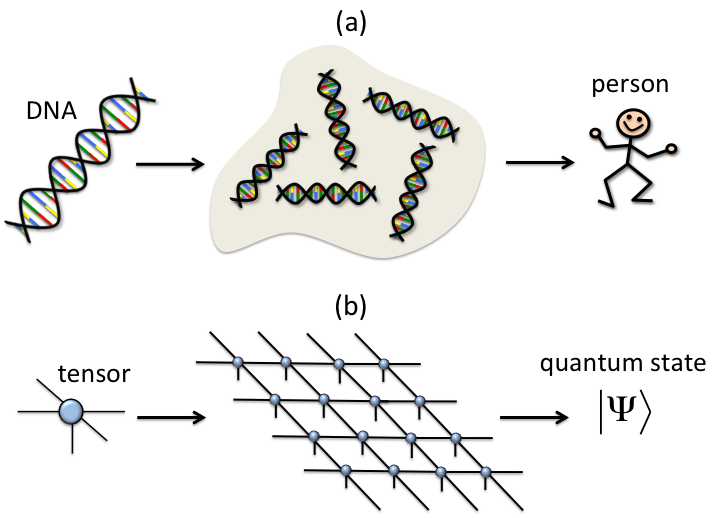
\includegraphics[width=0.99\linewidth]{cartoon.png}
\caption{Example of a figure from Ref.~\cite{Orus2013}.}
\label{fig:example}
\end{figure}
% \section{Разделы}

Начинаем с introduction, потом Results, Theoretical Background, Methods, Discussion, Appendices

Хочется донести мысли про MI, что вот он такой существует, что у него вот такие свойства и их так можно использовать в эксперименте. По таким наблюдаемым можно судить о том что у вас получилось выйти на MI. 

Хочется рассказать про dmrg, как расширение mean field, для этого показываем переход по D от MF к точному решению. 

Ещё на это можно смотреть как на некоторую демонстрацию методов. Посмотрим на проекцию ps1 на ps2 от параметров. 
% % Lorem ipsum dolor sit amet, consectetur adipisicing elit, sed do eiusmod
% tempor incididunt ut labore et dolore magna aliqua. Ut enim ad minim veniam,
% quis nostrud exercitation ullamco laboris nisi ut aliquip ex ea commodo
% consequat. Duis aute irure dolor in reprehenderit in voluptate velit esse
% cillum dolore eu fugiat nulla pariatur. Excepteur sint occaecat cupidatat non
% proident, sunt in culpa qui officia deserunt mollit anim id est laborum.
% \begin{equation*}
% 	\ket{\psi} = \alpha_1 \raisebox{-6.3mm}{
\includegraphics[width=0.08\textwidth]{s1.pdf}} + 
% 	\alpha_2 \raisebox{-6.3mm}{
\includegraphics[width=0.08\textwidth]{s2.pdf}} + 
% 	\alpha_3 \raisebox{-6.3mm}{
\includegraphics[width=0.08\textwidth]{s3.pdf}} + \ldots
% \end{equation*}

% \begin{equation*}
% 	\hat{H} = J \sum_{\langle i,j\rangle} \hat{S}_i \hat{S}_j - t \sum_{\langle i,j\rangle} \hat{c}_i\D \hat{c}_j
% \end{equation*}

% \begin{equation*}
% 	f(z) = \left\{\begin{aligned}
% 	    &1 - {\tilde{N}^0_{\text{pred}> z}}/{\tilde{N}^1_{\text{pred}< z}}, &z \geq \text{treshold} \\
% 	    &{\tilde{N}^1_{\text{pred}< z}}/{\tilde{N}^0_{\text{pred}> z}}-1, &z < \text{treshold} \\
% 	\end{aligned}\right.
% \end{equation*}


% \begin{equation*}
% 	f(z) = \tilde{N}^1_{\text{pred}< z}
% \end{equation*}


%  \begin{equation*}
%  	\hat{H} = - \sum_{\langle i,j\rangle} \hat{c}_i\D \hat{c}_j
%  \end{equation*}

%  \begin{equation*}
%  	g_2(r) = \langle \hat{c}_{\vc{j}}\D \hat{c}_{\vc{j}+\vc{r}}\D \hat{c}_{\vc{j}+\vc{r}}\hat{c}_{\vc{j}}\rangle_{\vc{j}}
%  \end{equation*}

%  \begin{equation*}
%  	\sub{\hat{H}}{FH} = - t \sum_{\langle i,j\rangle, \sigma} \hat{c}_{i \sigma}\D \hat{c}_{j \sigma} + U \sum_j \hat{n}_{j \uparrow} \hat{n}_{j \downarrow} + \sum_{j, \sigma} (V_j - \mu)\hat{n}_{j, \sigma}
%  \end{equation*}

%  \begin{equation*}
%  	{\hat{H}}_{tJ} = - t \sum_{\langle i,j\rangle, \sigma} \hat{c}_{i \sigma}\D \hat{c}_{j \sigma} + J \sum_{\langle i,j\rangle}\left(
%  		\hat{S}_i \hat{S}_j - \tfrac{1}{4} n_i n_j
%  	\right) + O(t^3 / U^2)
%  \end{equation*}

%  \begin{equation*}
%  	\langle \hat{O}\rangle(T) = \tfrac{1}{Z}\sum_j e^{- E_j / T} \bk{\psi_j}[\hat{O}]{\psi_j}
%  \end{equation*}

% \begin{equation*}
% {\hat{H}}_{tJ} = - t \sum_{\langle i,j\rangle, \sigma} \hat{c}_{i \sigma}\D \hat{c}_{j \sigma} + J \sum_{\langle i,j\rangle}
% 	\hat{S}_i \hat{S}_j
% \end{equation*}

% Stern-Gerlach: $F = \mu_z  \cdot \tfrac{\partial B}{\partial z} $



% \begin{equation*}
% 	\begin{pmatrix}
% 		\text{cost}_1 \\ \ldots \\ \text{cost}_n
% 	\end{pmatrix} \to \begin{pmatrix}
% 		w_1 \cdot \text{cost}_1 \\ \ldots \\ w_n \cdot  \text{cost}_n
% 	\end{pmatrix} 
% \end{equation*}


% \section{Code}

Какой код писать? Наверное кусочек из python, кусочек из Julia, 


% \bibliography{DMRG}




\end{document}







